\section{Auswertung}
	\label{sec:auswertung}

	\subsection{Filterkurve des Selektivverst"arkers} % (fold)
	\label{sub:subsection_name}
	
	Die Untersuchung der Filterkurve des Selektiv-Verst"arkers ergab die in Tabelle \ref{tabelle:aufgabe_a} aufgelisteten Werte.
	Daraus ergibt sich der Graph \ref{graph:aufgabe_a}.
	Aus diesem lassen sich die Werte f"ur $\nu_\mathrm{0}$, $\nu_\mathrm{+}$ und $\nu_\mathrm{-}$ ablesen:

	\begin{eqnarray*}
		\nu_\mathrm{0} &=& \SI{34.9}{\kilo\hertz} \\
		\nu_\mathrm{+} &=& \SI{35.10 (2)}{\kilo\hertz}\\
		\nu_\mathrm{-} &=& \SI{34.72 (2)}{\kilo\hertz}
	\end{eqnarray*}

	Aus diesen l"asst sich die G"ute mithilfe von Gleichung \eqref{Gleichung:Guete} berechnen.

	\begin{equation*}
		Q = \SI{91.84 (684)}{}
	\end{equation*}

	Der Fehler ergibt sich mittels Gau"s'scher Fehlerfortpflanzung:

	\begin{eqnarray*}
		|\frac{\partial Q}{\partial\nu_\mathrm{+}}| &=& |\frac{\partial Q}{\partial\nu_\mathrm{-}}| \\
		\Delta \nu_\mathrm{+} &=& \Delta \nu_\mathrm{-} \\
		\Delta Q &=& \sqrt{ 2 \cdot \left( |\frac{\partial Q}{\partial\nu_\mathrm{+}}| \Delta \nu_\mathrm{+,-} \right)^2}
	\end{eqnarray*}

	Damit weicht die errechnete G"ute Q = $\SI{91.84 (684)}{}$ um etwa $\SI{8.8}{\%}$ von der eingestellten G"ute Q = $100$ ab.

	\begin{table}[!h]
\begin{center}
\begin{tabular}{|r|r|r|r|}
\hline
f[$\SI{}{\kilo\hertz}$] & U[$\SI{}{\milli\volt}$] & f[$\SI{}{\kilo\hertz}$] & U[$\SI{}{\milli\volt}$]\\
\hline
\hline
25.0 &	0.0 &	35.1 &	6.1 \\	
30.0 &	0.2 &	35.2 &	4.9 \\	
30.5 &	0.2 &	35.3 &	4.0 \\	
31.0 &	0.3 &	35.4 &	3.4 \\	
31.5 &	0.4 &	35.5 &	2.9 \\	
32.0 &	0.5 &	35.6 &	2.5 \\	
32.5 &	0.6 &	35.7 &	2.2 \\	
33.0 &	0.7 &	35.8 &	2.0 \\	
33.5 &	1.1 &	35.9 &	1.8 \\	
34.0 &	1.8 &	36.0 &	1.6 \\	
34.1 &	2.0 &	36.5 &	1.1 \\	
34.2 &	2.3 &	37.0 &	0.8 \\	
34.3 &	2.7 &	37.5 &	0.6 \\	
34.4 &	3.1 &	38.0 &	0.5 \\	
34.5 &	3.8 &	38.5 &	0.4 \\	
34.6 &	4.6 &	39.0 &	0.3 \\	
34.7 &	5.9 &	39.5 &	0.3 \\	
34.8 &	7.4 &	40.0 &	0.2 \\	
34.9 &	8.6 &	40.5 &	0.0 \\	
35.0 &	7.4 &  & \\
\hline
\end{tabular}
\end{center}

	\begin{figure}[!h]
		\centering
		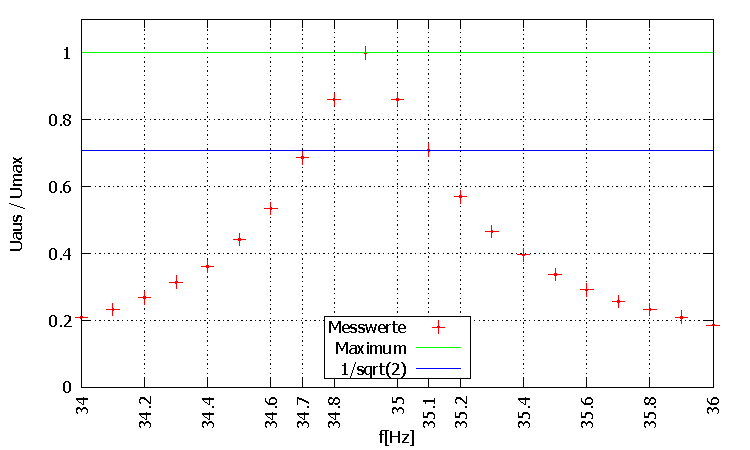
\includegraphics[width = 14cm]{img/arschlecken.pdf}
		\caption{Filterkurve des Selektivverst"arkers}
		\label{graph:aufgabe_a}
	\end{figure}